% !TEX program = xelatex
\documentclass[11pt, a4paper]{article}

\usepackage[top=2cm, bottom=2cm, left=2.5cm, right=2cm]{geometry}
\usepackage{fontspec}
\setmainfont{Times New Roman}
\setsansfont{Arial}
\setmonofont{Courier New}[Scale=0.95]
\usepackage{amsmath, amssymb}
\usepackage{booktabs}
\usepackage{tabularx}
\usepackage{graphicx}
\usepackage{float}
\usepackage{xcolor}
\usepackage{hyperref}
\usepackage{xurl}
\usepackage{parskip}
\usepackage{microtype}
\usepackage{caption}
\usepackage{enumitem}
\usepackage{fvextra}
\usepackage{tikz}
\usetikzlibrary{positioning, arrows.meta, calc}

\graphicspath{{../results/figures/}}
\newcommand{\restable}[1]{\input{../results/tables/#1}}
\emergencystretch=10em

\hypersetup{
    colorlinks=true,
    linkcolor=blue!70!black,
    citecolor=blue!70!black,
    urlcolor=blue!70!black,
    pdftitle={Agent 02 - RL-Based Agents versus Rule-Based Agents},
    pdfauthor={Nguyen Van Truong}
}

\DefineVerbatimEnvironment{codeblock}{Verbatim}{breaklines, breakanywhere, frame=single, framesep=2mm,
    fontsize=\small, rulecolor=\color{gray!60}}
\newcommand{\code}[1]{\texttt{#1}}
\setlist{itemsep=2pt, topsep=4pt}
\newcommand{\question}[2]{\subsection*{Question #1. #2}\addcontentsline{toc}{subsection}{Question #1. #2}}

\begin{document}

% ---------------------------------------------------------
% COVER PAGE
% ---------------------------------------------------------
\begin{titlepage}
\begin{center}

\vspace*{0.5cm}

\Large
\textbf{POSTS AND TELECOMMUNICATIONS INSTITUTE OF TECHNOLOGY}\\
\textbf{Faculty of Information Technology}

\vspace{2.0cm}

\Huge
\textbf{Intelligent System Development}\\
\vspace{0.4cm}
\LARGE
\textbf{LABORATORY EXPERIMENT 02 (AGENT 02)}\\
\vspace{0.6cm}
\Large
\textbf{Reinforcement-Learning-Based Agents\\versus Rule-Based Agents\\in a Simulated E-commerce Market}

\vspace{1.2cm}

\vfill

\normalsize
\begin{tabular}{rl}
\textbf{Lecturer:} & Assoc. Prof. Dinh Que Tran, Ph.D. \\
\textbf{Email:} & quetd@ptit.edu.vn, tdque@yahoo.com \\[0.8cm]
\textbf{Student Name:} & Nguyễn Văn Trường \\
\textbf{Student ID:} & B23DCCE095 \\
\textbf{Class:} & E23CNPM02 \\
\textbf{Semester:} & I.2025 -- 2026 \\
\textbf{Submission:} & Individual Project \\
\end{tabular}

\vfill

\textbf{Hanoi, 2026}

\vspace{0.5cm}

\end{center}
\end{titlepage}

{\small\tableofcontents}
\newpage

% =====================================================================
\section{Introduction and Objectives}

Two online shops sell the same product. At every time step each shop decides whether to offer a 20\% discount. A discount attracts more buyers but leaves less profit on each sale, and it also takes buyers away from the other shop. This laboratory builds that market as a small simulation and puts two kinds of decision maker into it:

\begin{itemize}
    \item a \textbf{reinforcement-learning (RL) agent} that starts with no knowledge and learns, from the profit it earns, which action is worth more in each situation (tabular Q-learning);
    \item a \textbf{rule-based agent} that follows three \emph{if--then} rules written by a person and never changes them.
\end{itemize}

The objectives, taken from the assignment, are to explain the concepts of agent, environment, state, action, reward and policy; to implement both agents and a two-agent simulation; to measure them with the same metrics; and to explain the limits of learning-based and rule-based decisions.

\textbf{What this report adds to the reference code.} The provided reference program trains the RL agent against the rule-based agent and evaluates it once. I kept its environment, Q-learning update and rule unchanged, and added what is needed to draw conclusions that hold up (Section~\ref{sec:setup}): an evaluation in which both agent types sit in the \emph{same seat} against the \emph{same opponent} on the \emph{same demand sequence}; ten independent seeds for every configuration; exploration settings with fixed $\varepsilon$; and three extra experiments that answer Questions 8--10 with measurements instead of opinion.

\textbf{Main findings in one paragraph.} Under the reference model the best a shop can do against the rule-based rival is never to discount (expected profit 35 per step), and the rule-based agent already does exactly that. The RL agent reaches the same policy in 8 of 10 seeds, but in the other 2 it keeps discounting in a situation where that is a mistake, so on average it earns slightly less (34.39 vs 34.97 per step). The reasons can be measured: a constant learning rate keeps the Q-values noisy, and the state hides the delayed reaction of the rival. When the market changes (an aggressive rival or other opponents), the fixed rules lose up to 4.5 units per step against the best response, while RL agents stay within about 0.1--1 unit of it. An improved agent trained against a pool of opponents with a decreasing step size was the most robust of all agents tested.

% =====================================================================
\section{Environment and Agents}
\label{sec:model}

\subsection{The market as a multi-agent environment}

Figure~\ref{fig:loop} shows one time step. Both agents observe their local state, choose an action \emph{at the same time} without seeing the other's choice, and the environment returns a profit to each and a new state.

\begin{figure}[H]
\centering
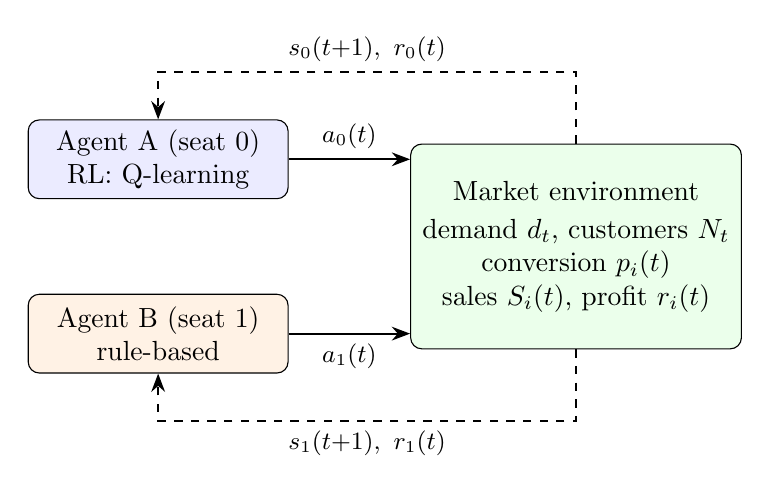
\begin{tikzpicture}[node distance=1.2cm and 2.4cm, >=Stealth,
    box/.style={draw, rounded corners, align=center, minimum width=3.3cm, minimum height=1.0cm, fill=#1},
    box/.default=white]
\node[box=blue!8] (rl) {Agent A (seat 0)\\RL: Q-learning};
\node[box=orange!10, below=of rl] (rule) {Agent B (seat 1)\\rule-based};
\node[box=green!8, right=3.2cm of $(rl)!0.5!(rule)$, minimum height=2.6cm, minimum width=4.2cm] (env) {Market environment\\[2pt] demand $d_t$, customers $N_t$\\ conversion $p_i(t)$\\ sales $S_i(t)$, profit $r_i(t)$};
\draw[->, thick] (rl.east) -- node[above, sloped, font=\small]{$a_0(t)$} (env.west |- rl.east);
\draw[->, thick] (rule.east) -- node[below, sloped, font=\small]{$a_1(t)$} (env.west |- rule.east);
\draw[->, thick, dashed] (env.north) |- node[pos=0.75, above, font=\small]{$s_0(t{+}1),\ r_0(t)$} ($(rl.north)+(0,0.6)$) -- (rl.north);
\draw[->, thick, dashed] (env.south) |- node[pos=0.75, below, font=\small]{$s_1(t{+}1),\ r_1(t)$} ($(rule.south)+(0,-0.6)$) -- (rule.south);
\end{tikzpicture}
\caption{One step of the two-agent market. Solid arrows: simultaneous actions. Dashed arrows: rewards and next states.}
\label{fig:loop}
\end{figure}

\begin{description}[leftmargin=0pt]
    \item[State.] Agent $i$ observes $s_i(t) = (d_t, c_i(t))$: demand $d_t \in \{0, 1\}$ (low, high) and the competitor's \emph{previous} action $c_i(t) \in \{0, 1\}$. Four states per agent.
    \item[Action.] $a_i(t) \in \{0, 1\}$: no discount or discount.
    \item[Conversion.] Each of the $N_t$ potential customers buys with probability
    $p_i(t) = \mathrm{clip}\big(0.30 + 0.25 d_t + 0.15 a_i(t) - 0.10 a_{-i}(t),\ 0.05,\ 0.95\big)$, where $a_{-i}(t)$ is the competitor's \emph{current} action.
    \item[Reward.] $N_t = 10$ (low demand) or $20$ (high). Sales $S_i(t) \sim \mathrm{Binomial}(N_t, p_i(t))$. Price $P=10$, cost $C=5$, discount $\delta = 0.2$. Profit $r_i(t) = S_i(t)\,\big(P(1-\delta a_i(t)) - C\big)$, i.e.\ 5 per sale without and 3 per sale with a discount.
    \item[Transition.] Next demand is drawn uniformly at random, independently of the actions; each agent's current action becomes the competitor's previous action. An episode has 20 steps and starts with both previous actions set to 0.
\end{description}

\subsection{What the model implies}

Before running anything it helps to know what a good policy looks like. Multiplying customers, conversion probability and margin gives the expected one-step profit (Table~\ref{tab:expected}).

\begin{table}[H]
\centering
\caption{Expected one-step profit $E[r] = N_t\, p_i\, (\text{margin})$ for every demand level and competitor action (computed by \code{expected\_profit}).}
\label{tab:expected}
\restable{expected_profit.tex}
\end{table}

Not discounting is better in three of the four cases. The only case where a discount pays (low demand while the rival discounts, $+0.5$) never happens against the reference rule, because the rule never discounts when demand is low. A discount also has a \emph{delayed} cost: the rule discounts at the next step if demand is high and we discounted now, which lowers our next profit by 10 (from 55 to 45). So against the rule-based rival the best policy is \textbf{never discount}, with expected profit $0.5 \times 15 + 0.5 \times 55 = 35$ per step. This number is the benchmark used throughout. If neither agent ever discounts, both earn 35.

\subsection{Agent A: tabular Q-learning}

The RL agent stores one value $Q(s, a)$ for each of the $4 \times 2 = 8$ state--action pairs, initialised to zero. It picks actions $\varepsilon$-greedily (random action with probability $\varepsilon$, otherwise the action with the larger $Q$; ties broken at random) and after each step applies
\[
Q(s_t, a_t) \leftarrow Q(s_t, a_t) + \alpha \Big[ r_t + \gamma \max_{a} Q(s_{t+1}, a) - Q(s_t, a_t) \Big],
\]
with the target reduced to $r_t$ at the last step of an episode. The reference values are $\alpha = 0.10$, $\gamma = 0.90$ and $\varepsilon_{\text{episode}} = \max(0.02,\ 0.20 \cdot 0.995^{\text{episode}})$.

\begin{codeblock}
def learn(self, state, action, reward, next_state, terminal=False):
    d, c = state
    nd, nc = next_state
    old_value = self.q[d, c, action]
    target = reward if terminal else reward + self.gamma * np.max(self.q[nd, nc])
    self.visits[d, c, action] += 1
    alpha = 1.0 / self.visits[d, c, action] if self.step_size == "visit" else self.alpha
    self.q[d, c, action] = old_value + alpha * (target - old_value)
\end{codeblock}

The \code{step\_size="visit"} branch is used only by the improved agent of Question~10; with the default \code{"constant"} the update is exactly the reference one.

\subsection{Agent B: rule-based}

\[
\pi^{\text{rule}}(d, c) =
\begin{cases}
0, & d = 0 \quad\text{(low demand: no discount)},\\
1, & d = 1 \text{ and } c = 1 \quad\text{(high demand, rival discounted: match it)},\\
0, & d = 1 \text{ and } c = 0 \quad\text{(high demand, rival did not: no discount)}.
\end{cases}
\]

\begin{codeblock}
class RuleBasedAgent:
    is_learner = False
    def act(self, state, explore=True):
        demand, competitor_previous_action = state
        if demand == 0:
            return NO_DISCOUNT
        elif demand == 1 and competitor_previous_action == 1:
            return DISCOUNT
        else:
            return NO_DISCOUNT
    def learn(self, *args, **kwargs):
        pass        # a rule-based agent does not learn from rewards
\end{codeblock}

% =====================================================================
\section{Experimental Setup}
\label{sec:setup}

\subsection{Program structure}

Everything is in one file, \code{code/agent02\_experiment.py} (NumPy and Matplotlib only, no GPU). It contains the environment class, the Q-learning agent, the rule-based agent and a few extra opponents, one \code{train} function, one \code{evaluate} function and one function per experiment. Running \code{python agent02\_experiment.py} rebuilds every CSV file, figure and table in this report in about 25 minutes on a laptop; the tables in this report are \verb|\input| directly from the files the script writes, so no number was copied by hand.

\subsection{Parameters and seeds}

\begin{table}[H]
\centering
\caption{Parameters. All reference values are kept unless an experiment changes one of them.}
\begin{tabular}{ll}
\toprule
Parameter & Value \\
\midrule
Agents & 2 (seat 0: agent under test, seat 1: opponent) \\
Training episodes $\times$ steps & 5{,}000 $\times$ 20 = 100{,}000 steps \\
Learning rate $\alpha$ / discount factor $\gamma$ & 0.10 / 0.90 \\
Exploration & $\varepsilon = \max(0.02,\ 0.20 \cdot 0.995^{\text{episode}})$ \\
Price / unit cost / discount & 10 / 5 / 20\% \\
Baseline seed (Experiments A, B) & 42 for the environment, 42 + 10{,}000 for the agent \\
Repeated runs (Experiments C--E, Q8--Q10) & seeds 11, 22, \dots, 110 (10 seeds) \\
Evaluation & 500 episodes (10{,}000 steps), $\varepsilon = 0$, no learning \\
Evaluation seed & training seed + 800{,}000 (baseline: 42 + 500{,}000) \\
Learning-curve window & $K = 100$ episodes \\
\bottomrule
\end{tabular}
\end{table}

\subsection{Evaluation protocol}

The reference training loop measures reward while the agent is still exploring and learning, which mixes two things. Evaluation is therefore a separate run: the Q-table is frozen, $\varepsilon = 0$, and a new environment is created with its own seed.

\textbf{Fair comparison.} The two agents do not play symmetric roles in the reference experiment: the RL agent in seat 0 faces the rule, and so does the rule-based agent in seat 1, but each faces a different opponent behaviour. To compare the two \emph{policies}, I evaluate both of them in seat 0 against the same rule-based opponent with the same evaluation seed: \emph{RL vs Rule} and \emph{Rule vs Rule}. The environment draws exactly one demand value and two binomial samples per step whatever the actions are, so both runs see the identical demand sequence and the same random stream (common random numbers). Any difference in reward then comes from the policies alone.

\begin{codeblock}
def evaluate(config, agent0, agent1, seed, episodes=None):
    env = ECommerceEnvironment(config, seed=seed)     # separate evaluation seed
    ...
    for ep in range(episodes):
        states = env.reset()
        for _ in range(T):
            actions = [agents[i].act(states[i], explore=False) for i in range(2)]
            states, rewards, _ = env.step(actions)    # no learn() call: Q is frozen
            ...
\end{codeblock}

\textbf{Metrics.} The average reward of agent $i$ over $T$ steps, $\overline{R}_i = \frac{1}{T}\sum_{t=1}^{T} r_i(t)$; total reward; number of discount and no-discount actions; the learned Q-table and greedy policy; for learning curves, the mean reward per step over windows of $K = 100$ episodes, $\overline{R}_{i,k} = \sum_{t \in \mathcal{W}_k} r_i(t) / (20K)$. Across seeds I report the mean and the sample standard deviation of $\overline{R}_i$, and how many of the 10 seeds ended with a greedy policy that never discounts.

% =====================================================================
\section{Results}

\subsection{Experiment A: baseline (seed 42)}

\begin{table}[H]
\centering
\caption{Separate greedy evaluation of the baseline agents: 500 episodes, 10{,}000 steps, evaluation seed 42 + 500{,}000.}
\label{tab:baseline}
\resizebox{\textwidth}{!}{\restable{baseline_eval.tex}}
\end{table}

\begin{table}[H]
\centering
\caption{Learned Q-table of the baseline RL agent after 5{,}000 training episodes (seed 42). Visits are counted over the whole training run.}
\label{tab:qtable}
\restable{baseline_qtable.tex}
\end{table}

\textbf{Observations.}
\begin{itemize}
    \item In evaluation the RL agent never discounts, and its total reward (351{,}275) equals that of the rule-based agent in the same seat to the last unit. The two policies take identical actions on every one of the 10{,}000 steps, which confirms both that the comparison is paired correctly and that RL found the benchmark policy for this seed.
    \item The greedy policy (Table~\ref{tab:qtable}) is ``no discount'' in the two states with $c = 0$ and ``discount'' in the two with $c = 1$. The second part looks like the rule's ``match the rival'' behaviour, but those states are visited only 4\% of the time during training (2{,}501 + 1{,}522 and 3{,}468 + 409 visits out of 100{,}000) and \emph{never} in greedy evaluation, because the rival only discounts after we do. The policy in those states is therefore weakly learned and irrelevant here.
    \item During training (with exploration) the totals were 3{,}345{,}548 for RL and 3{,}283{,}930 for the rule-based agent, i.e.\ 33.46 and 32.84 per step. RL took a discount on 17.5\% of training steps, the rule on 8.3\%. The rule discounts during training only because it reacts to RL's exploratory discounts, which shows how one agent's behaviour changes the other's outcome.
\end{itemize}

\subsection{Experiment B: the learning process}

\begin{figure}[H]
\centering
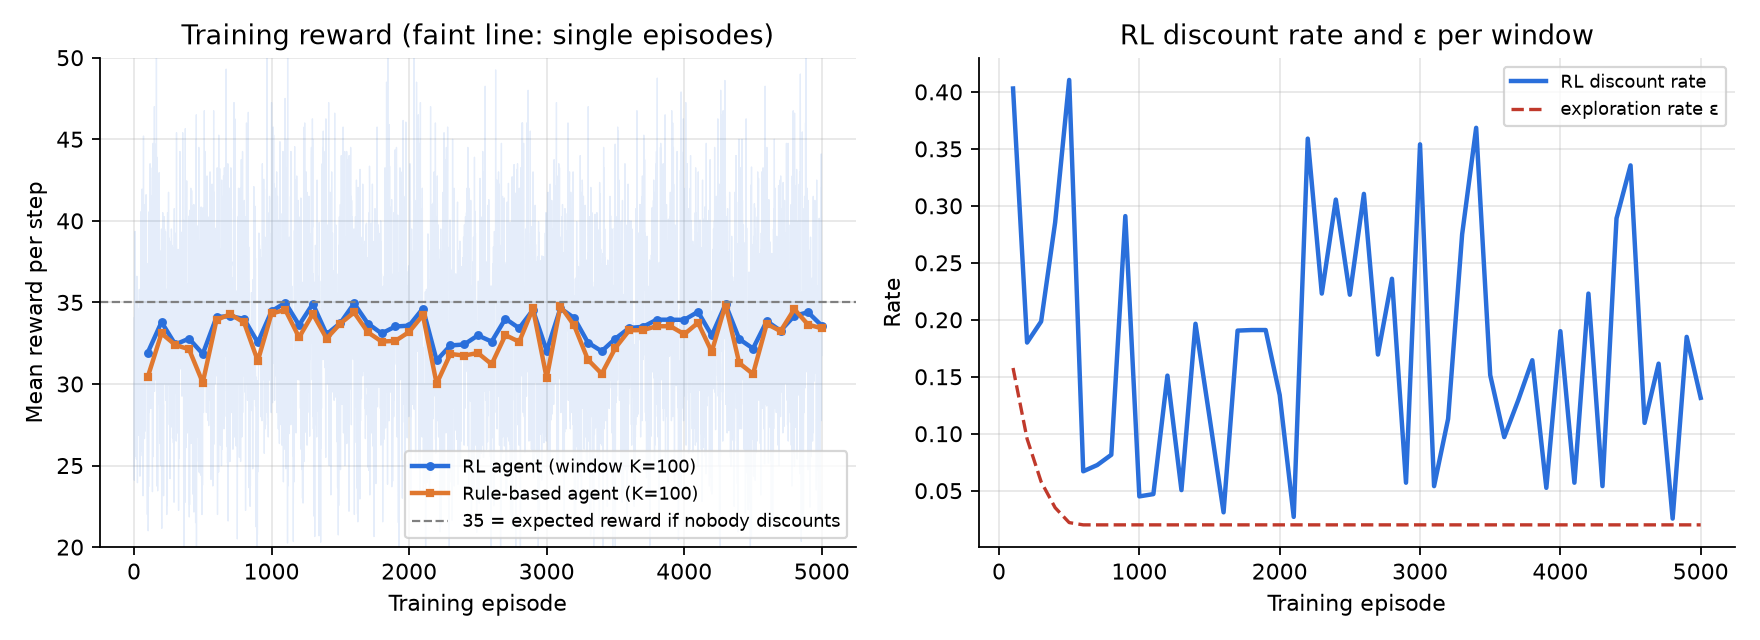
\includegraphics[width=\textwidth]{baseline_training.png}
\caption{Baseline training, seed 42. Left: mean reward per step for each episode (faint) and per window of $K = 100$ episodes. Right: share of steps on which RL discounted, and the exploration rate, per window.}
\label{fig:baseline-train}
\end{figure}

The windowed reward rises from about 32 in the first window to 33--35 after roughly 500 episodes, but it does not settle: it keeps moving between about 31 and 35 until the end (Figure~\ref{fig:baseline-train}). Single episodes range from about 20 to 50, because the demand of every step is random. The right panel explains the dips. Exploration reaches its floor of $\varepsilon = 0.02$ after about 460 episodes, so after that random exploration causes a discount on only 1\% of steps, yet the discount rate keeps jumping between 3\% and 37\%. Those discounts come from the \emph{greedy} policy itself: it switched 606 times during training (counting a switch whenever the greedy action of any state changed between two episodes). Each time the greedy action in state $(0,0)$ or $(1,0)$ flips to ``discount'', the rule reacts and both shops' rewards drop together, which is why the two curves move in parallel.

So the training reward \emph{improves early and then fluctuates}. A good-looking final window is not proof of convergence: the policy evaluated in Experiment A is a snapshot of a Q-table that is still changing. It happened to be the right snapshot for seed 42, but Experiment E shows it is not for every seed.

\subsection{Experiment C: learning rate}

\begin{table}[H]
\centering
\caption{Learning rate, 10 seeds each, other parameters unchanged. Train reward: mean over all 5{,}000 training episodes. ``Never discount'': seeds whose final greedy policy never discounts in any state. Policy changes: number of episodes after which the greedy policy differed from the previous one.}
\label{tab:lr}
\restable{learning_rate.tex}
\end{table}

\begin{figure}[H]
\centering
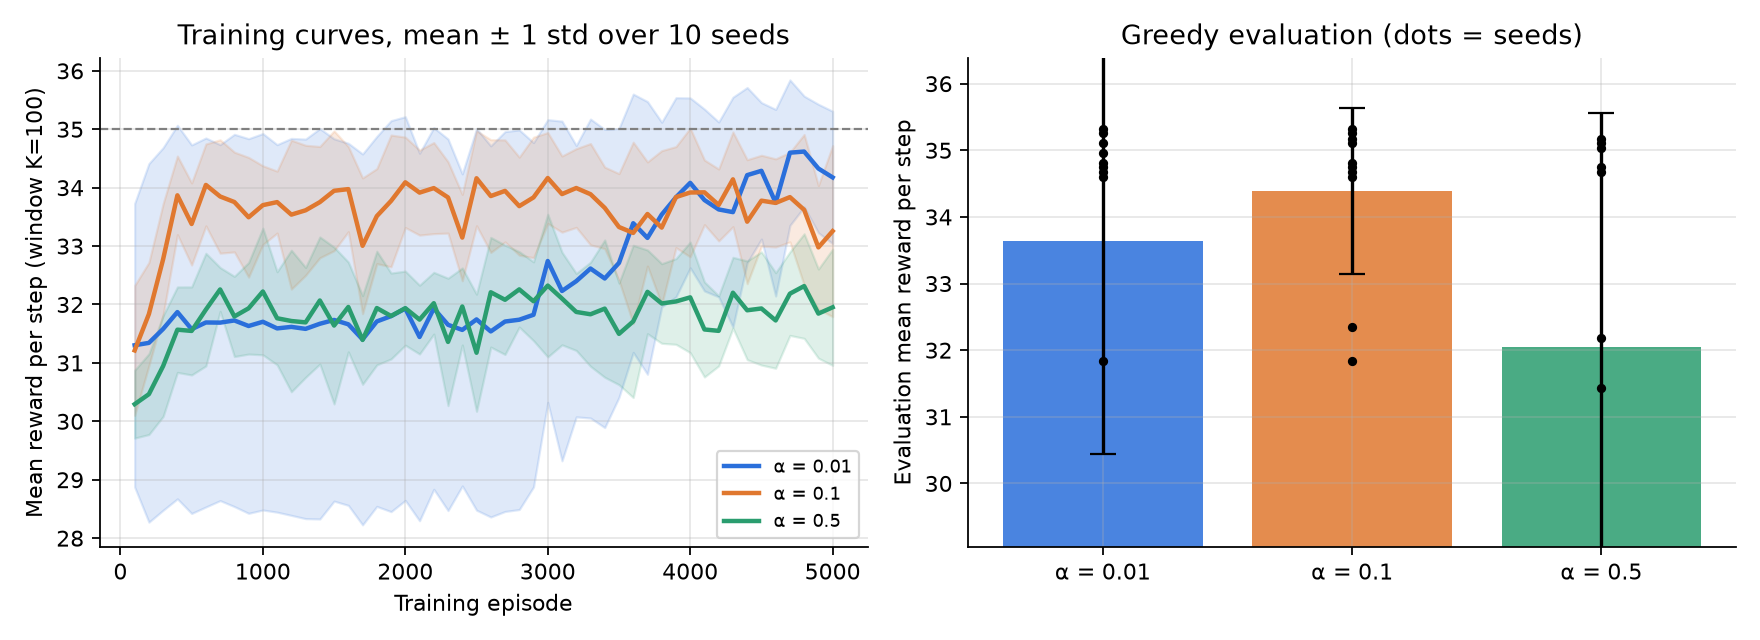
\includegraphics[width=\textwidth]{learning_rate_comparison.png}
\caption{Left: windowed training reward, mean $\pm$ 1 std over 10 seeds. Right: greedy evaluation reward, one dot per seed.}
\label{fig:lr}
\end{figure}

$\alpha = 0.10$ gives the best evaluation reward and by far the smallest spread across seeds. $\alpha = 0.01$ updates so slowly that the Q-values are still climbing from their initial 0 towards values of about 150--260 for much of the run. While they climb, the action that has been chosen more often has simply received more updates and looks better, so the greedy choice reinforces itself. For seed 11, for example, the agent took ``discount'' 31{,}019 times and ``no discount'' only 4{,}358 times in state $(0,0)$ before ``no discount'' finally overtook it. Its greedy policy changed only 21.5 times per run: it is stable, but often stable in the wrong place. $\alpha = 0.50$ reacts strongly to every new sample: its policy changed about 1{,}770 times per run (one change every three episodes), training reward is the lowest, and the final policy is close to a coin flip in the states where the two Q-values are near each other. Questions~6 and~7 discuss this further.

\subsection{Experiment D: exploration}

\begin{table}[H]
\centering
\caption{Exploration settings, 10 seeds each, $\alpha = 0.10$. Train and evaluation rewards are means over seeds; std is across seeds.}
\label{tab:exp}
\restable{exploration.tex}
\end{table}

\begin{figure}[H]
\centering
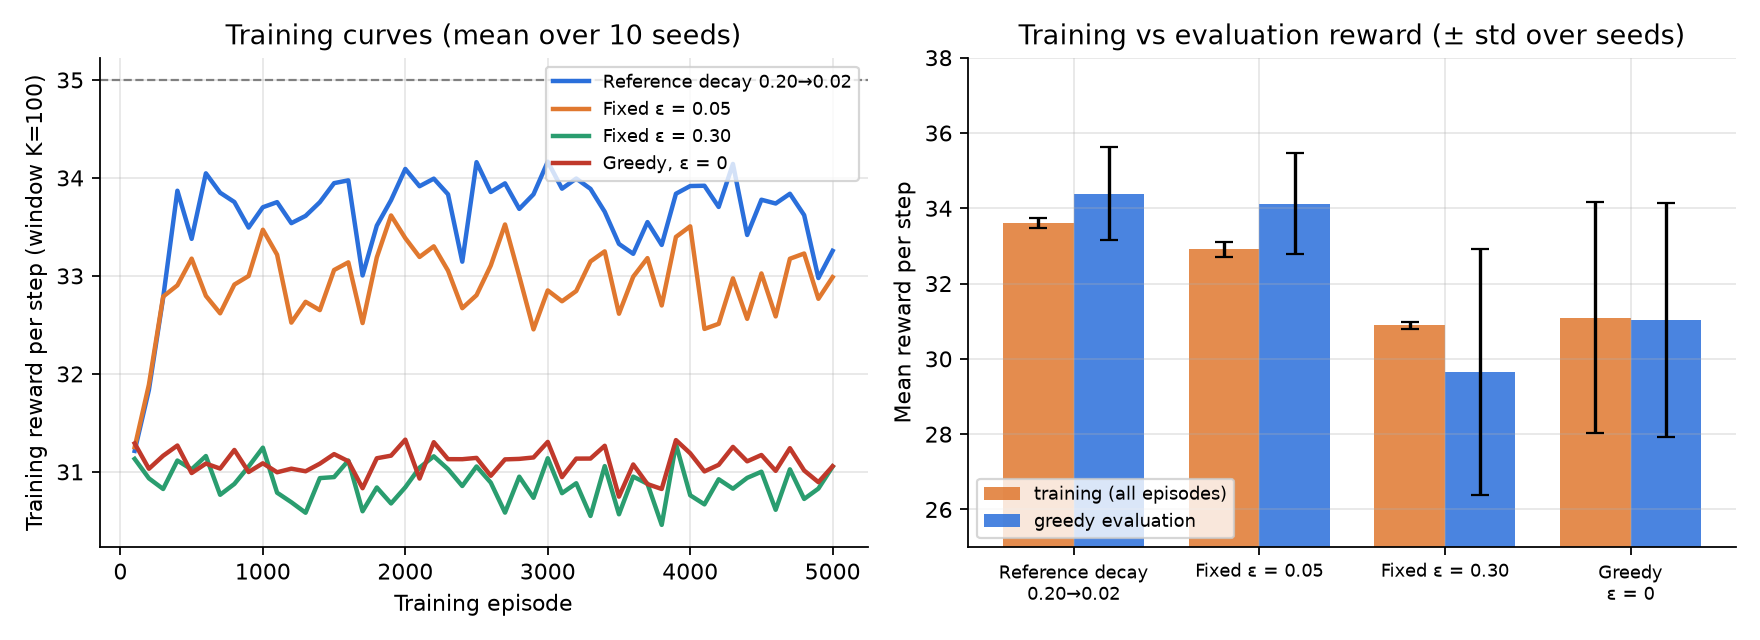
\includegraphics[width=\textwidth]{exploration_comparison.png}
\caption{Left: windowed training reward (mean over 10 seeds). Right: training reward vs greedy evaluation reward for each exploration setting.}
\label{fig:exp}
\end{figure}

The decaying reference schedule is best in both training and evaluation. A fixed $\varepsilon = 0.05$ is close in evaluation (34.12) but pays about 0.7 per step during training for its extra random actions. A fixed $\varepsilon = 0.30$ has the lowest training reward (30.89) and, surprisingly, an even lower evaluation reward (29.65): none of its 10 final policies is ``never discount''. The purely greedy agent ($\varepsilon = 0$) never changed its policy at all (0 changes): with all Q-values starting at 0 and every profit positive, the first action it tries in each state becomes the greedy action forever. Its result depends entirely on the seed (std 3.07). Question~4 explains these effects.

\subsection{Experiment E: fair comparison over 10 seeds}

\begin{table}[H]
\centering
\caption{Results table (Section 7.6 of the assignment). Every agent is in seat 0 against the reference rule-based opponent; greedy evaluation over 500 episodes per seed; mean and std across 10 seeds. Discount rate: share of evaluation steps with a discount.}
\label{tab:results}
\resizebox{\textwidth}{!}{\restable{results_table.tex}}
\end{table}

\begin{figure}[H]
\centering
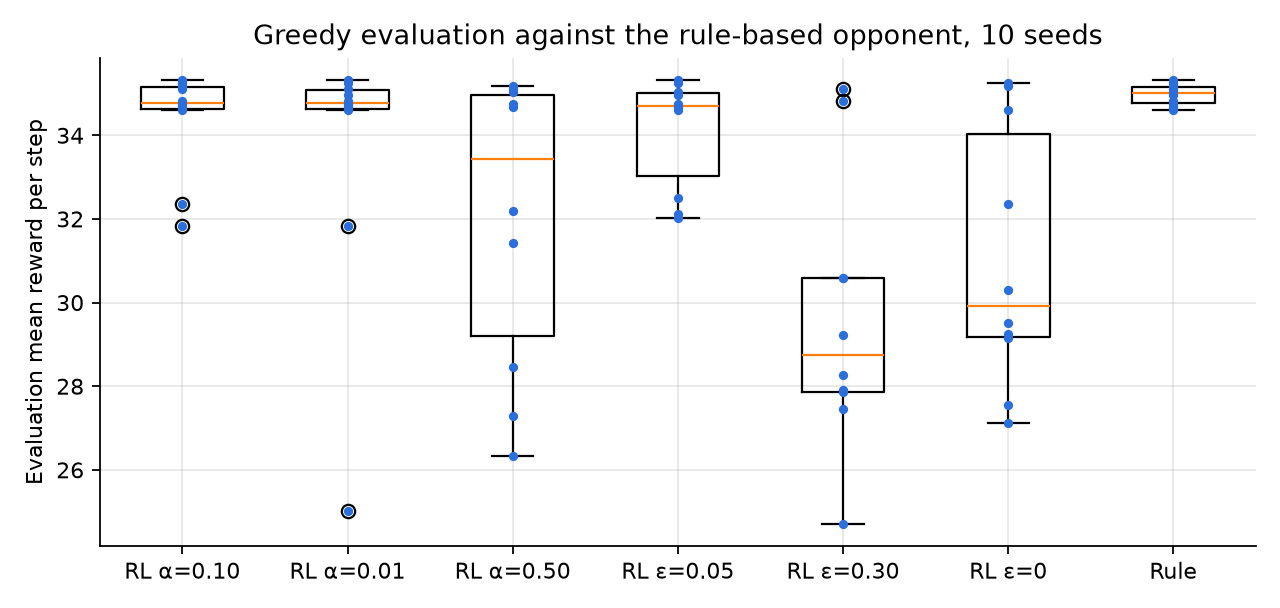
\includegraphics[width=0.85\textwidth]{multi_seed_comparison.png}
\caption{Greedy evaluation reward of every configuration against the rule-based opponent; each dot is one seed.}
\label{fig:multi}
\end{figure}

The rule-based agent earns 34.97 $\pm$ 0.25 per step, in line with the expected 35. Its spread across seeds comes only from random demand and sales, since its policy is fixed. The best RL configuration (the reference) earns 34.39 $\pm$ 1.24. Because the comparison is paired (same seeds, same demand), I also computed the per-seed difference RL $-$ Rule: it is exactly 0 for 8 seeds and $-3.19$ and $-2.61$ for seeds 66 and 77 (mean $-0.58$, std 1.23). So RL either matches the rule-based policy or does worse; it never does better, which is expected because the rule already plays the best response. Only 4 of the 10 RL policies are ``never discount'' in \emph{all} four states, but the other 4 that still earn the same reward discount only in the unreachable states with $c = 1$.

% =====================================================================
\section{Answers to the Ten Laboratory Questions}

\question{1}{Agent and environment modeling}

\begin{itemize}
    \item \textbf{Agents:} two sellers. Seat 0 is the agent under test (the Q-learning agent); seat 1 is the opponent (the rule-based agent in the reference set-up).
    \item \textbf{Environment:} the market, i.e.\ the customers, the random demand, the conversion and profit rules and the record of last step's actions (\code{ECommerceEnvironment}).
    \item \textbf{State space:} $\mathcal{S} = \{0,1\} \times \{0,1\}$, demand and the competitor's previous action: $(0,0), (0,1), (1,0), (1,1)$.
    \item \textbf{Action space:} $\mathcal{A} = \{0, 1\}$, no discount or discount.
    \item \textbf{Reward:} the profit of the step, $r_i = S_i \big(P(1-\delta a_i) - C\big)$, with $S_i \sim \mathrm{Binomial}(N_t, p_i)$.
    \item \textbf{Transition:} $d_{t+1}$ is uniform on $\{0,1\}$ independently of everything; $c_i(t+1) = a_{-i}(t)$.
\end{itemize}

\textbf{Why it is a multi-agent system.} Each seller's reward depends on the other seller's \emph{current} action (the $-0.10\,a_{-i}$ term) and its next state contains the other's action. A single-agent model would have to treat the rival as part of the environment. That only works if the rival never changes behaviour; as soon as it reacts to us (the rule matches our discount) or learns (Question~8), the ``environment'' changes with our own choices. Modelling two agents makes this interaction explicit and lets us study strategic effects: in Experiment A, the rule discounted on 8.3\% of training steps purely in reaction to RL's exploratory discounts.

\question{2}{Learning-based versus rule-based decisions}

\begin{table}[H]
\centering
\small
\begin{tabularx}{\textwidth}{lXX}
\toprule
 & RL agent (Q-learning) & Rule-based agent \\
\midrule
Decision making & Picks the action with the higher learned value $Q(s,a)$; occasionally explores. & Looks up the action in three hand-written rules. \\
Use of experience & Every step updates $Q$; behaviour changes with data. & Ignores rewards; behaviour never changes. \\
Adaptability & Re-learns a good response when the market changes (Q9: RL retrained earns 28.76 vs 27.84 for the rule). & Must be rewritten by a developer when the market changes. \\
Computation & 100{,}000 training steps (about 10 s here) and an 8-entry table; much more for large state spaces. & No training; one comparison per decision. \\
Predictability & Different seeds give different policies (std 1.24 across seeds). & Identical decisions every time; easy to audit. \\
\bottomrule
\end{tabularx}
\end{table}

\textbf{A rule-based agent is preferable} when the right behaviour is known and must be guaranteed, explained or audited, or when there is no safe way to experiment. Example: a legally required price floor, or ``never sell below cost'', or a new shop with no sales history to learn from. In the reference market the rule happens to be the best response and RL can only match it.

\textbf{An RL agent is preferable} when the best response is unknown or keeps changing and experimentation is cheap. Example: a marketplace seller facing many competitors whose pricing strategies change each season. In the robustness test of Question~10, learning agents earned 1.1--1.7 more per step on average across five rival types than the fixed rule.

\question{3}{Q-learning update}

The update moves the current estimate $Q(s,a)$ a fraction $\alpha$ of the way towards a \emph{target}: the reward just received plus the discounted value of the best action in the next state. The bracket $r + \gamma \max_{a'} Q(s',a') - Q(s,a)$ is the \emph{temporal-difference (TD) error}: positive if the outcome was better than expected, negative if worse.

With $Q(s,a) = 4$, $\alpha = 0.1$, $r = 6$, $\gamma = 0.9$ and $\max_{a'} Q(s',a') = 5$:
\begin{align*}
\text{target} &= r + \gamma \max_{a'} Q(s',a') = 6 + 0.9 \times 5 = 6 + 4.5 = 10.5,\\
\text{TD error} &= 10.5 - 4 = 6.5,\\
\text{change} &= \alpha \times 6.5 = 0.1 \times 6.5 = 0.65,\\
Q_{\text{new}}(s,a) &= 4 + 0.65 = 4.65.
\end{align*}

\textbf{Interpretation.} The action turned out better than the agent believed (10.5 against 4), so its value increases, but only by 10\% of the gap, to 4.65. One lucky outcome is not trusted completely; repeated good outcomes keep pushing the value up. With $\alpha = 1$ the value would jump to 10.5 at once; with $\alpha = 0.01$ it would only reach 4.065.

\question{4}{Exploration and exploitation}

$\varepsilon$-greedy selection takes a random action with probability $\varepsilon$ (exploration) and otherwise the action with the higher $Q$-value (exploitation). Exploration is needed because a Q-value can only improve if the action is actually tried; exploitation is needed to earn reward with what has been learned. The experiments (Table~\ref{tab:exp}) show both failure modes:

\begin{itemize}
    \item \textbf{Exploring too much ($\varepsilon = 0.30$ fixed).} Training reward drops to 30.89 (from 33.61) because 15\% of steps are random discounts and each one also triggers the rule's retaliation at the next high-demand step. Worse, the \emph{learned} policy is also poor (evaluation 29.65, discount rate 0.49, no seed reached ``never discount''). The random discounts make the rival's next action vary unpredictably, so the targets the agent learns from are much noisier, and with $\alpha = 0.10$ the small difference between the two actions in low demand is swamped by this noise. The greedy policy changed 2{,}429 times per run.
    \item \textbf{Stopping exploration too early ($\varepsilon = 0$).} With zero initial values and positive profits, whichever action is tried first in a state gets a positive value and is chosen forever (0 policy changes). In 3 of 10 seeds that first choice was ``no discount'' everywhere and the agent did well; in the others it locked in discounting somewhere and lost up to 8 per step (27.11 for the worst seed). Mean 31.03 with std 3.10: the outcome is luck, not learning.
    \item \textbf{The reference decay} explores widely in the first 500 episodes and then exploits with $\varepsilon = 0.02$. It gave the best training (33.61) and evaluation (34.39) reward. A small fixed $\varepsilon = 0.05$ learns almost as well (34.12) but keeps paying for exploration during training (32.91).
\end{itemize}

\question{5}{Reward and business objectives}

A discount lowers the price, so more visitors buy (conversion $+0.15$), but every sale earns less. With $P = 10$, $C = 5$, $\delta = 0.20$:
\begin{align*}
\text{no discount:}\quad & 10 - 5 = 5 \text{ per sale},\\
\text{discount:}\quad & 10 \times (1 - 0.20) - 5 = 8 - 5 = 3 \text{ per sale}.
\end{align*}
The margin falls by 40\%, so a discount only pays if sales rise by at least $5/3 \approx 1.67$ times. The conversion gain of $+0.15$ is far below that: $0.30 \to 0.45$ in low demand is $\times 1.5$, and $0.55 \to 0.70$ in high demand only $\times 1.27$. That is why ``no discount'' wins in Table~\ref{tab:expected} except when the rival is already discounting in low demand.

\textbf{Changing the reward changes the behaviour.} The agent maximises whatever the reward measures, not what the business ``means''. For example:
\begin{itemize}
    \item \emph{Revenue instead of profit} ($r = S \cdot P_{\text{eff}}$): with 8 vs 10 per sale and $\times 1.27$--$1.5$ more sales, discounting becomes better in every state and the agent would learn to always discount.
    \item \emph{Profit plus a market-share bonus} ($r = \text{profit} + \lambda S$): for large enough $\lambda$ the extra sales outweigh the lost margin and the agent discounts more.
    \item \emph{A smaller discount}, e.g.\ $\delta = 0.10$ (margin 4): in low demand $10 \times 0.45 \times 4 = 18 > 15$ and in high demand $20 \times 0.70 \times 4 = 56 > 55$, so a myopic agent would always discount, and the outcome depends on whether the rival's retaliation (cost about $0.5 \times 8 \times \gamma$) outweighs the gain.
\end{itemize}

\question{6}{Performance evaluation}

Average reward per step, $\overline{R} = \frac{1}{T}\sum_t r(t)$, from the greedy evaluations ($T = 10{,}000$ steps per seed):

\begin{table}[H]
\centering
\small
\begin{tabular}{lrr}
\toprule
Measurement & RL agent & Rule-based agent \\
\midrule
Baseline, seed 42, same seat (Table~\ref{tab:baseline}) & 35.127 & 35.127 \\
Baseline, seed 42, the reference RL vs Rule match & 35.127 (seat 0) & 34.968 (seat 1) \\
Training phase, seed 42 (with exploration) & 33.455 & 32.839 \\
10 seeds, same seat, mean $\pm$ std (Table~\ref{tab:results}) & 34.390 $\pm$ 1.239 & 34.970 $\pm$ 0.253 \\
10 seeds, paired difference RL $-$ Rule & \multicolumn{2}{c}{$-0.580 \pm 1.231$ (0 in 8 seeds)} \\
\bottomrule
\end{tabular}
\end{table}

\begin{figure}[H]
\centering
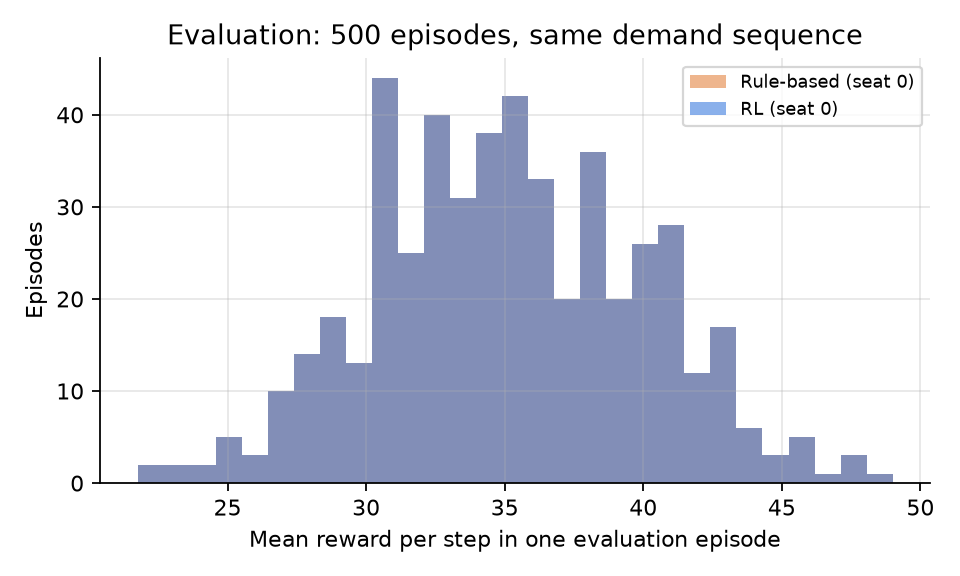
\includegraphics[width=0.6\textwidth]{baseline_eval_hist.png}
\caption{Distribution of the per-episode mean reward in the seed-42 evaluation. The two histograms coincide exactly because both policies took identical actions on the same demand sequence.}
\end{figure}

\textbf{Why one run is not enough.} Seed 42 alone would suggest that RL and the rule are identical (and the reference match even makes RL look 0.16 better, which is only the difference between the two seats' random sales). Ten seeds show that RL is worse in 2 of 10 runs by about 3 per step. Several sources of randomness change the result of a single run: the random demand and binomial sales (a single 20-step episode ranges from about 20 to 50 per step), the agent's own exploration and tie-breaking, and the moment at which training stops while the greedy policy is still switching (606 switches in the seed-42 run). A claim that one approach is \emph{generally} better also needs other market settings and opponents (Questions~9 and~10), not only other seeds.

\question{7}{Learning rate and stability}

The learning rate sets how much each new observation moves $Q$: after $n$ updates, the weight of an observation $k$ steps old is $\alpha (1-\alpha)^k$. With $\alpha = 0.5$ the latest few samples dominate; with $\alpha = 0.01$ the estimate averages over hundreds of samples. Measured over 10 seeds (Table~\ref{tab:lr}, Figure~\ref{fig:lr}):

\begin{itemize}
    \item \textbf{$\alpha = 0.01$: stable but slow.} Only 21.5 policy changes per run, but the values are still rising from 0 for much of training, so the action tried more often looks better simply because it has been updated more; evaluation 33.63 with the largest spread (3.19), and only 1 seed learned ``never discount''. Low sensitivity to new observations means low sensitivity to \emph{useful} information too.
    \item \textbf{$\alpha = 0.10$: the best compromise} (34.39 $\pm$ 1.24), though still 584 policy changes per run.
    \item \textbf{$\alpha = 0.50$: fast but unstable.} About 1{,}770 policy changes per run; training reward 31.81, evaluation 32.05 $\pm$ 3.51, discount rate 0.29. In low demand the true gap between the two actions is a few units while a single reward varies by about $\pm 7$, so a Q-value that half-resets to each new sample ranks the two actions almost at random.
\end{itemize}

Faster updating therefore did \emph{not} improve stability; it caused excessive fluctuation. A constant $\alpha$ in a noisy environment never stops fluctuating; a step size that decreases with the number of visits (used in Question~10) addresses this.

\question{8}{Multi-agent interaction and non-stationarity}

\textbf{Influence of the other agent.} The rival's \emph{current} action changes my conversion probability by $-0.10$, which costs 5 per step in low demand and 10 in high demand (Table~\ref{tab:expected}). The rival's \emph{previous} action is part of my state. Against the rule-based rival there is also a feedback loop: my discount now makes the rival discount at the next high-demand step, which lowers my next reward. This delayed cost is not visible in my state, which contains the rival's last action but not my own (see Question~9).

\textbf{Why independent Q-learning is hard when both learn.} Q-learning assumes the environment's transition and reward probabilities are fixed. If the rival also learns, the reward I get for the same $(s, a)$ changes as the rival's policy changes: the problem is \emph{non-stationary}. Old samples become wrong, the two agents chase each other, and convergence guarantees no longer hold.

\textbf{Experiment.} I trained two independent Q-learners against each other (same parameters, different random generators) and compared with RL against the fixed rule, over 10 seeds (Figure~\ref{fig:rlrl}).

\begin{figure}[H]
\centering
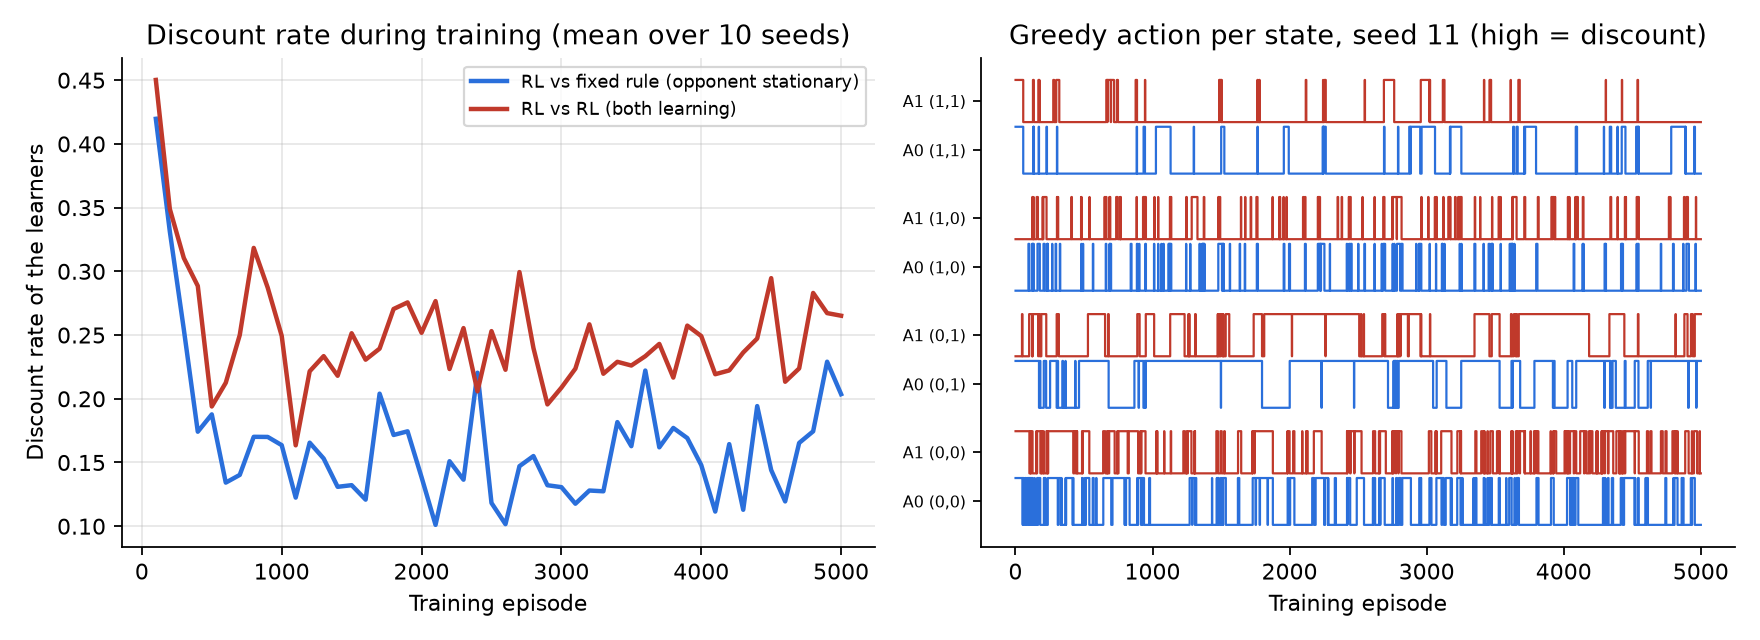
\includegraphics[width=\textwidth]{rl_vs_rl.png}
\caption{Left: share of steps with a discount during training, RL vs fixed rule and RL vs RL (mean over 10 seeds). Right: greedy action of each state over training for both learners (A0, A1), seed 11.}
\label{fig:rlrl}
\end{figure}

\begin{itemize}
    \item With two learners, the discount rate during training stays higher (about 0.20--0.30 instead of 0.10--0.20): each agent's exploratory discounts make the other's learned values noisier.
    \item In greedy evaluation of the two final policies against each other, 6 of the 10 pairs settled on ``nobody discounts'' (about 35 each), while 4 pairs ended with one or both still discounting (down to 29.1--29.9 for seed 33). Mean reward 33.63 $\pm$ 1.86 and 33.62 $\pm$ 2.01, lower and more variable than RL against the fixed rule.
    \item The number of policy changes was almost the same (589 vs 584 per run). In this tiny problem the noise from a constant $\alpha$ already causes most of the instability, so this counter cannot separate the two effects. This is an honest limitation of the measurement.
\end{itemize}

\textbf{An experimental change to study the problem further:} freeze one learner while the other learns, alternating every $M$ episodes. If performance and stability improve as $M$ grows, non-stationarity is the cause. A second option is to give each agent the rival's recent action frequencies in the state, so changes in the rival's behaviour become observable.

\question{9}{Limitations and robustness}

\textbf{Limitations of the reference simulation.}
\begin{enumerate}
    \item \textbf{Demand is i.i.d.} (a fair coin each step), with no trend, seasonality or persistence, and cannot be influenced by prices. Real demand is autocorrelated, so the state should carry more history.
    \item \textbf{The conversion formula is illustrative}: linear, the same for every customer, with fixed effects of $+0.15$ and $-0.10$. Customers cannot switch shops or remember earlier prices, and the binomial noise is large relative to the differences between actions.
    \item \textbf{The state is incomplete.} The rule reacts to \emph{my} previous action, but that action is not in my state, and the step within the 20-step episode is not either (yet the value of the future depends on how many steps remain). The problem is therefore not exactly a Markov decision process from the agent's point of view.
    \item \textbf{Only one fixed opponent and two actions}: the agent is trained and tested against the same rule, so the measurement says nothing about other rivals; prices are binary (0\% or 20\%).
    \item \textbf{Short training and a single objective}: profit per step only, with no inventory, cost of changing prices or long-term customer value.
\end{enumerate}

\textbf{Implemented modification: an aggressive competitor.} I replaced the rival's rule with ``discount whenever demand is high'', a plausible change in a real market. Against this rival, never discounting is still the best response, with expected profit $0.5 \times 15 + 0.5 \times 45 = 30$. The reference rule-based agent, however, sees ``high demand and rival discounted last step'' on 25\% of steps, matches the discount and earns 36 instead of 45 on those steps; expected value $30 - 0.25 \times 9 = 27.75$.

\begin{table}[H]
\centering
\caption{Modified market: aggressive competitor in seat 1. Greedy evaluation, 10 seeds.}
\label{tab:mod}
\resizebox{\textwidth}{!}{\restable{modification.tex}}
\end{table}

\textbf{Effect on the results.} The measured rule-based reward (27.84) agrees with the calculation (27.75), and its ``match the rival'' rule, harmless in the reference market, now loses about 2.2 per step. On average both RL agents beat it: the agent retrained in the new market by $+0.92 \pm 1.20$ per step on average (paired over seeds: better in 6 of 10 seeds, equal in 1, slightly worse in 3) and the agent trained in the old market and moved unchanged by $+1.47$. Neither reached the optimum of 30 reliably: the retrained agent still discounted on 32\% of steps on average, for the same reasons as in Experiment E (noisy values with a constant $\alpha$). The two RL variants differ by less than one standard deviation, so the data do not show that retraining helped here. The change in the ranking, however, is clear: a rule that fits one market can be the worst choice in another, while a learning agent adapts without a developer rewriting it.

\question{10}{Design a better intelligent agent}

\textbf{Proposed agent.} The experiments point to three weaknesses of the reference agent: values stay noisy because $\alpha$ is constant, it has seen only one opponent, and its state hides its own previous action. The proposed agent addresses each:

\begin{itemize}
    \item \textbf{State:} $(d_t, c_t, a_{t-1})$: demand, the rival's last action and the agent's own last action, so the delayed reaction of a rival is observable (16 Q-values). Further extensions: a demand trend, the rival's discount frequency over the last $k$ steps, the steps left in the episode.
    \item \textbf{Actions:} discount or not (could be extended to several discount levels).
    \item \textbf{Reward:} profit per step, as in the business objective (Question~5 explains why not revenue).
    \item \textbf{Learning:} Q-learning with a step size $\alpha = 1/N(s,a)$ that shrinks with the number of visits, so values average out the sales noise instead of fluctuating, and training against a \textbf{pool of opponents} (rule, aggressive, tit-for-tat, always discount, random), one drawn at random each episode.
    \item \textbf{Evaluation:} greedy and frozen; against every opponent type separately; 10 seeds; report mean, std, the \emph{worst case} across opponents and the gap to the best response computed from the model.
\end{itemize}

\textbf{Test of robustness.} I implemented the proposal in two steps, opponent pool with $\alpha = 1/N$, then also the extended state, and evaluated all agents against five opponents (Table~\ref{tab:robust}).

\begin{table}[H]
\centering
\caption{Robustness test: mean reward per step $\pm$ std over 10 seeds, greedy evaluation against each opponent. Last row: best expected reward against that opponent computed from the model.}
\label{tab:robust}
\resizebox{\textwidth}{!}{\restable{robustness.tex}}
\end{table}

\begin{itemize}
    \item The \textbf{rule-based agent} is optimal against the rule and tit-for-tat, but loses 4.5 per step against an always-discounting rival (23.23 vs 27.75), because it then matches the rival's discount even in high demand.
    \item The \textbf{reference RL agent}, trained only against the rule, already transfers better (average 31.08, worst 26.70) but is noisy (std up to 1.74).
    \item \textbf{Opponent pool + $\alpha = 1/N$} is the most robust: average 31.59 and worst case 27.53, within 0.1--0.3 of the best response against each opponent (31.80 and 27.75), with std of 0.22--0.24 against stateless rivals. Against the rule-based rival it earns 34.72, closer to 35 than the reference RL agent (34.42).
    \item \textbf{Adding the own previous action did not help} (average 31.21, and 34.02 against the rule). The hypothesis that the hidden delayed reaction is the main problem is therefore \emph{not} supported by this measurement. A likely explanation, not yet tested: the 16-entry table splits the same data over twice as many entries, and with $\alpha = 1/N$ early bootstrapped targets keep a long-lasting weight. Testing that would need longer training or a decaying $\alpha = 1/N^{0.6}$.
\end{itemize}

A limitation of this test: all five evaluation opponents were also in the training pool, so it measures robustness to \emph{known} rival types. A stricter test would hold one type out of training and evaluate against it.

So the agent I would recommend is the 8-state Q-learner trained against an opponent pool with a decreasing step size. It is more robust than the reference RL agent against every opponent, and more robust than the rule-based agent in average and worst case, while losing only 0.26 per step to the rule in the one market the rule was designed for.

% =====================================================================
\section{Discussion}

\textbf{Consistency vs quality of rules.} The rule-based agent was the most consistent agent in every test (std 0.14--0.27, coming only from random demand). Its performance, though, depended entirely on whether its rules suited the rival: best possible against the reference rule, 4.5 per step below the best response against an always-discounting rival.

\textbf{Learning does not guarantee an optimal policy.} The RL agent found the optimal policy in 8 of 10 seeds and never exceeded the rule, which was already optimal. A constant learning rate, a short horizon of very noisy rewards and an incomplete state meant that the greedy policy kept changing until training stopped.

\textbf{Randomness.} The same fixed policy earns 34.97 $\pm$ 0.25 over ten seeds and single episodes range from 20 to 50 per step. Paired evaluation (common random numbers) removed this noise from the RL-vs-rule comparison: on seed 42 the two totals were identical to the last unit.

\textbf{Interacting learners.} Two learners influence each other's data: the rule discounted 8.3\% of training steps only because of RL's exploration, and with two learners 4 of 10 pairs ended in a worse joint outcome.

\textbf{Training vs evaluation.} The two measure different things. With $\varepsilon = 0.30$, training reward was 30.89 and evaluation 29.65; with the reference schedule, 33.61 and 34.39. A training curve shows how much the agent earned \emph{while} learning, including the cost of exploration; only a frozen, separate evaluation shows the quality of the learned policy.

\textbf{Observation vs explanation.} The numbers in this report are observations. Explanations given as such (``noise from a constant $\alpha$'', ``the hidden delayed reaction'') are supported by indirect evidence, the number of policy changes and the visit counts, but are not proven. One of them, that the hidden own action is the main problem, was tested in Question~10 and not confirmed.

% =====================================================================
\section{Conclusion}

I implemented the two-seller market, a tabular Q-learning agent and a rule-based agent, and compared them with a separate, paired, multi-seed evaluation. In the reference market the hand-written rule is already the best response, and Q-learning reaches the same policy in most runs (34.39 $\pm$ 1.24 vs 34.97 $\pm$ 0.25 per step). The learning rate and exploration schedule matter: $\alpha = 0.10$ with decaying $\varepsilon$ worked best, while too much exploration, no exploration, too slow or too fast learning all produced worse and less reliable policies. When the rival changes, the advantage reverses: fixed rules lose up to 4.5 per step and learning agents adapt. An agent trained against a pool of opponents with a decreasing step size came within 0.3 per step of the best response against every opponent tested. The broader lesson is that the winner depends on the market: which agent is better is a question about the environment and its assumptions as much as about the algorithm.

% =====================================================================
\section*{Reproducibility}
\addcontentsline{toc}{section}{Reproducibility}

\begin{codeblock}
pip install numpy matplotlib
cd agent_02/code
python agent02_experiment.py               # all experiments (~25 min), writes ../results/
python agent02_experiment.py robustness    # only the Question 10 experiment
cd ../report && xelatex agent02_E23CNPM02_truongnv_095.tex   # run twice for the contents
\end{codeblock}

Python 3.13, NumPy 2.5, Matplotlib 3.11. The notebook \code{notebook/agent02\_demo.ipynb} runs the same experiments step by step with explanations. Seeds and the evaluation protocol are listed in Section~\ref{sec:setup}. All CSV files (per-seed and summary) are in \code{agent\_02/results/}.

\section*{References}
\addcontentsline{toc}{section}{References}

\begin{enumerate}[label={[\arabic*]}]
    \item Intelligent System Development, \emph{Laboratory Experiment 02: Reinforcement-Learning-Based Agents versus Rule-Based Agents}, assignment and reference implementation (\code{agent02\_experiment.py}), 2026.
    \item R. S. Sutton and A. G. Barto, \emph{Reinforcement Learning: An Introduction}, 2nd ed., MIT Press, 2018 (Q-learning, $\varepsilon$-greedy, step-size parameters).
\end{enumerate}

\end{document}
